%------------------------------------------------------------------------------------
%	CHAPTER 2
%------------------------------------------------------------------------------------
\chapterimage{headSpark.png}
\chapter{Primeiros Exemplos}

\begin{remark}
"Inovação é a faísca que acende o fogo da mudança e impulsiona o progresso da tecnologia." (Bill Gates) 
\end{remark}

\section{Meu Hello World?}\index{Primeiros Exemplos}
Como todo nosso ambiente montado vamos criar um novo caderno, a primeira ação que devemos realizar é criar uma seção e um contexto para conversação com o Spark. Importamos a biblioteca necessária:
\begin{lstlisting}[]
from pyspark.sql import SparkSession
\end{lstlisting}

Criamos o objeto de seção:
\begin{lstlisting}[]
spark = SparkSession.\
        builder.\
        appName("pyspark-notebook").\
        master("spark://spark-master:7077").\
        config("spark.executor.memory", "512m").\
        getOrCreate()
\end{lstlisting}

Damos um nome para esta seção: \textbf{pyspark-notebook}, indicamos aonde está o Spark Master (conforme o contêiner Docker): spark-master:7077 e quanta memória deve utilizar: 512 Mb. Agora se voltarmos ao gerenciador veremos que os \textbf{Spark Workers} foram alocados para responder a essa seção:
\begin{figure}[H]
	\centering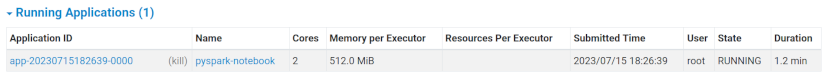
\includegraphics[scale=1.0]{cap02/WorkerAlocado}
	\caption{Seção Running Applications do Spark Master}
\end{figure}

Por fim criamos um contexto de conversação:
\begin{lstlisting}[]
sc = spark.sparkContext
\end{lstlisting}

Com essa célula executando perfeitamente temos o nosso Hello Wolrd pronto! Concordo, não teve a menor graça e parece que ficou faltando algo, bem wm paralelismo é assim mesmo que acontece, mas vamos em frente e verificarmos o que são objetos RDD.

\section{Objeto RDD}\index{Primeiros Exemplos}
Por definição, cada aplicativo \textbf{Spark} consiste em um programa que executa várias operações paralelas em um \textbf{cluster}. A abstração principal que \textbf{Spark} oferece é um conjunto chamado \textbf{RDD} (\textit{Resilient Distributed Dataset}), este é uma coleção de elementos particionados nos nós do \textbf{cluster}. Os RDDs são criados a partir de um arquivo no sistema de arquivos \textbf{Hadoop} (ou qualquer outro sistema de arquivos compatível com Hadoop). As características deste são:
\begin{figure}[H]
	\centering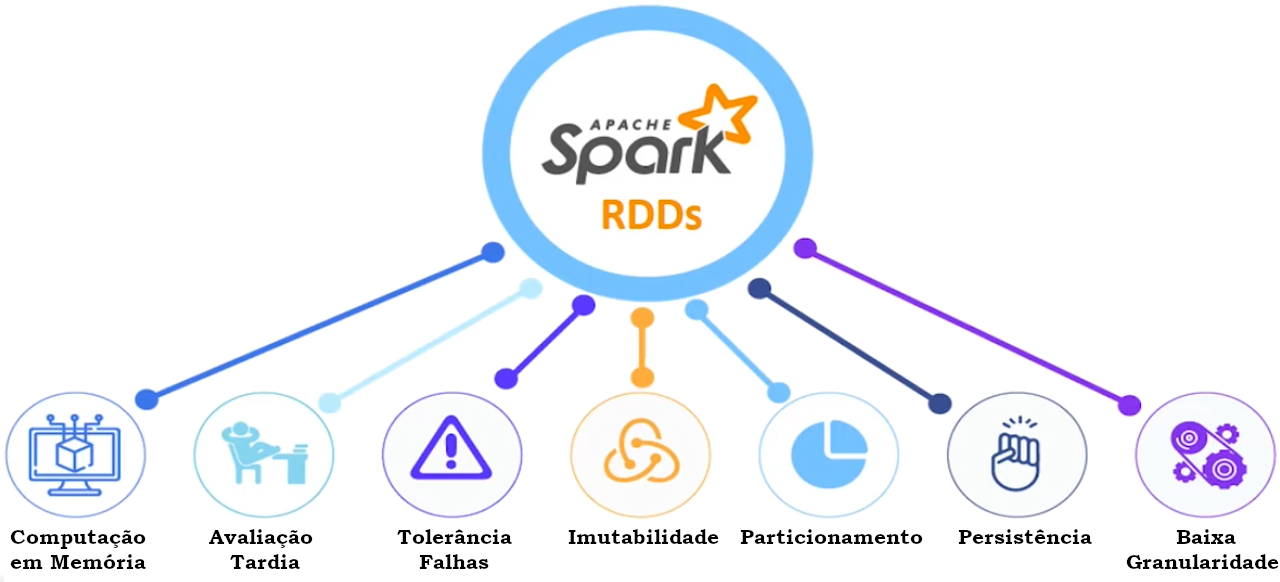
\includegraphics[scale=0.3]{cap02/ArquiteturaRDD}
	\caption{Características do RDD}
\end{figure}

Podem ser mantidos em memória, são trabalhados de forma tardia (Lazy, assim não alocam recursos do programa principal), possuem tolerância a falhas, são objetos imutáveis, são particionados, podem realizar persistência dos dados (guardá-los para recuperação posterior) e possuem baixa granularidade (coarse-grained service) e reduz o número de chamadas necessárias para concluir uma tarefa.

Vamos criar um RDD de forma bem simples através de uma lista:
\begin{lstlisting}[]
rdd = sc.parallelize([1,2,3,4,5,6,7,8,9,10])
print(type(rdd))
\end{lstlisting}

E como resposta temos: \\
{\ttfamily <class 'pyspark.rdd.RDD'>}

Para vermos os elementos usamos a função collect():
\begin{lstlisting}[]
print(rdd.collect())
\end{lstlisting}

E temos como resposta: \\
{\ttfamily [1, 2, 3, 4, 5, 6, 7, 8, 9, 10]}

\section{Uso de Arquivos Texto}\index{Primeiros Exemplos}
Também podemos ler um arquivo texto, para este exemplo criar um arquivo texto na mesma pasta com o nome: teste.txt e seguinte conteúdo:
\begin{lstlisting}[]
Apache Spark é um mecanismo de análise unificado para processamento de dados em grande escala.
Fornece APIs para linguagens de alto nível como Java, Scala, Python e R
Permite um mecanismo otimizado para suporte a gráficos de execução geral.
Possui um excelente conjunto de ferramentas, tais como:
    Spark SQL para SQL e processamento de dados estruturados;
    MLlib para aprendizado de máquina;
    GraphX para processamento de gráfico; e
    Streams estruturados para computação incremental e processamento de fluxo.
\end{lstlisting}

Para ler este arquivo usamos:
\begin{lstlisting}[]
rdd = sc.textFile('teste.txt')
print(type(rdd))
\end{lstlisting}

E observamos que é o mesmo tipo do objeto criado anteriormente, se desejar contar quantos elementos temos:
\begin{lstlisting}[]
print(rdd.count())
\end{lstlisting}

E retorna que temos 8 elementos, como assim? Spark utiliza as linhas como elementos, se quisermos verificar como o RDD foi montado é só usar o método collect()
\begin{lstlisting}[]
print(rdd.collect())
\end{lstlisting}

Obtemos toda sua configuração utilizada com o comando:
\begin{lstlisting}[]
print(sc.getConf().getAll())
\end{lstlisting}

Temos elementos que atrapalham nossos próximos passos, assim para remover vírgulas, dois pontos, ponto final e outros sinais de pontuação do texto em um RDD utilizamos as funções para a manipulação de strings disponíveis no Spark, importamos para isso a biblioteca \textbf{re}:
\begin{lstlisting}[]
import re
\end{lstlisting}

E para substituir esses caracteres por espaços em branco ou removê-los completamente
\begin{lstlisting}[]
rdd_sem_pontuacao = rdd.map(lambda linha: re.sub(r'[^\w\s]', '', linha))
for linha in rdd_sem_pontuacao.collect():
    print(linha)
\end{lstlisting}

Utilizamos a biblioteca do Python para utilizar a função \textbf{sub} e substituir os sinais de pontuação por espaços em branco. A expressão regular mostrada corresponde a qualquer caractere que não seja alfanumérico (w) ou espaço em branco (s).

Dessa forma, a transformação \textbf{map} é aplicada em cada linha do RDD para substituir os sinais de pontuação por espaços em branco. Em seguida, utilizamos o método \textbf{collect()} para coletar e imprimir todas as linhas do RDD sem pontuação.E temos como resultado as linhas livres de pontuação.

Agora podemos contar a quantidade de ocorrências para cada palavra no texto, porém ainda temos um pequeno problema que são as palavras sem significado próprio como "e", "é", "de" e por aí vai. vamos removê-las então:
\begin{lstlisting}[]
# Definir a lista de palavras indesejadas
palavras_indesejadas = ["e", "é", "um", "para", "em", "como", "a", "tais", "como", "de", ""]

# Dividir cada linha em palavras e criar um RDD com todas as palavras
palavras = rdd_sem_pontuacao.flatMap(lambda linha: linha.split(" "))

# Filtrar as palavras indesejadas
palavras_filtradas = palavras.filter(lambda palavra: palavra not in palavras_indesejadas)

# Contar as ocorrências de cada palavra
contagem_palavras = palavras_filtradas.countByValue()

# Imprimir as palavras únicas e suas contagens
print("Palavras únicas encontradas e suas contagens:")
for palavra, contagem in contagem_palavras.items():
    print(palavra, "->", contagem)
\end{lstlisting}

Definimos uma lista de palavras que desejamos remover da contagem. Em seguida, aplicamos o método \textbf{filter()} no \textbf{RDD} que não contém a pontuação usando uma condição lambda e assim filtrar as palavras que não estão presentes na lista de palavras indesejadas.

Contamos as ocorrências das palavras filtradas e imprimimos as palavras únicas encontradas e suas respectivas contagens.

\section{PipelinedRDD e DataFrame}\index{Primeiros Exemplos}
Quando falamos de \textbf{Pipeline} rapidamente associamos ao \textbf{Jenkins} e \textbf{DataFrame} ao \textbf{Pandas}, porém devemos esquecer essa associação aqui, o \textbf{PipelinedRDD} e uma subcoleção de um \textbf{RDD} e o \textbf{DataFrame} é o modo como Spark realiza uma associação de linhas e colunas.

Vamos imaginar que temos uma lista de 1.000 pacientes no qual colhemos os dados de Pressão Arterial, tanto a sistólica (PAS) quanto a diastólica (PAD). Para simularmos esses dados vamos importar a classe Random:
\begin{lstlisting}[]
import random
\end{lstlisting}

E criamos um método de modo a retornar os valores como uma lista:
\begin{lstlisting}[]
def valorPressao(x):
    idt = x
    pas = random.randint(11, 20)
    pad = random.randint(70, 121)
    return (x, pas, pad)
\end{lstlisting}

Definimos para PAS um valor aleatório porém devemos nos manter entre 11 e 19 e para PAD entre 70 e 121 de modo a criarmos dados viáveis. Agora criamos um objeto PipelinedRDD:
\begin{lstlisting}[]
rdd_pipe = sc.parallelize(range(1000)).map(valorPressao)
print(type(rdd_pipe))
\end{lstlisting}

E como resposta temos: \\
{\ttfamily <class 'pyspark.rdd.PipelinedRDD'>}

Podemos visualizar os 10 primeiros registros com:
\begin{lstlisting}[]
rdd_pipe.take(10)
\end{lstlisting}

E transformá-lo em um DataFrame com:
\begin{lstlisting}[]
df = rdd_pipe.toDF(("Id", "PAS", "PAD"))
type(df)
\end{lstlisting}

E como resposta temos: \\
{\ttfamily pyspark.sql.dataframe.DataFrame}

E visualizarmos os registros com:
\begin{lstlisting}[]
df.show()
\end{lstlisting}

Para encerramos o trabalho, não devemos esquecer de sempre fechar a seção, antes mesmo de parar a composição Docker.
\begin{lstlisting}[]
spark.sparkContext.stop()
\end{lstlisting}

E notamos na página de status do \textbf{Spark Master} que os \textbf{Spark Workers} alocados foram para a seção \textbf{Completed Applications}.
\clearpage